\vspace{-0.25cm}
\section{Evaluation}

We evaluate \framework{} on a set of image processing and stencil benchmarks.  We compare it with two other compilers: Halide\cite{halide_12}, 
an industrial-quality DSL for image processing that has a scheduling language, and PENCIL~\cite{pencil_paper}, a state-of-the-art fully automatic polyhedral compiler.

We performed the evaluation on a cluster of 16 nodes. Each node is a dual-socket machine with two 24-core Intel Xeon E5-2680v3 CPUs, 128 GB RAM, Ubuntu 14.04, and an Infiniband interconnect.  We use the MVAPICH2 2.0 \cite{mvapich2} implementation of MPI for the distributed tests.
%We use \emph{multicore} to refer to experiments performed on a single-node with multicores and \emph{distributed} to refer to a cluster of 16 nodes.
GPU experiments are performed on an NVIDIA Tesla K40 with 12 GB of RAM.  Each experiment is repeated $30\times$ and the median time is reported.

We used the following benchmarks in our evaluation: \texttt{edgeDetector}, a ring blur followed by Roberts edge detection~\cite{roberts65}; \texttt{cvtColor}, which converts an RGB image to grayscale; \texttt{convolution}, a simple 2D convolution; \texttt{warpAffine}, which does affine warping on an image;  \texttt{gaussian}, which performs a gaussian blur; \texttt{nb}, a synthetic pipeline composed of 4 stages that computes a negative and a brightened image from the same input image; and \texttt{ticket \#2373}, a code snippet from a bug filed against Halide where the inferred bounds are over-approximated, causing the generated code to fail due to an assertion during execution.
Four of these benchmarks have non-affine array accesses and non-affine conditionals for clamping (to handle boundary cases): \texttt{edgeDetector}, \texttt{convolution}, \texttt{warpAffine} and \texttt{gaussian}.
We used a $2112\times3520$ RGB input image for the experiments.
%The size of the filters range from 1 statement (for \texttt{cvtColor}) to 33 statements (for \textt{warpAffine}).
%performs a calculation Halide cannot currently support.  %For each of the benchmarks, we implement them both in Halide (when possible) and Halide-\framework{} and compare the performance.

% We implemented each one of the image processing benchmarks in Halide.  We compile these benchmarks using the original Halide compiler and measure the execution time (we call this compiler Halide-original), then we compile the benchmarks using a modified version of the Halide compiler which uses the \framework framework and measure the execution time (we call this compiler Halide-\framework).

\begin{figure}[t]
\centering
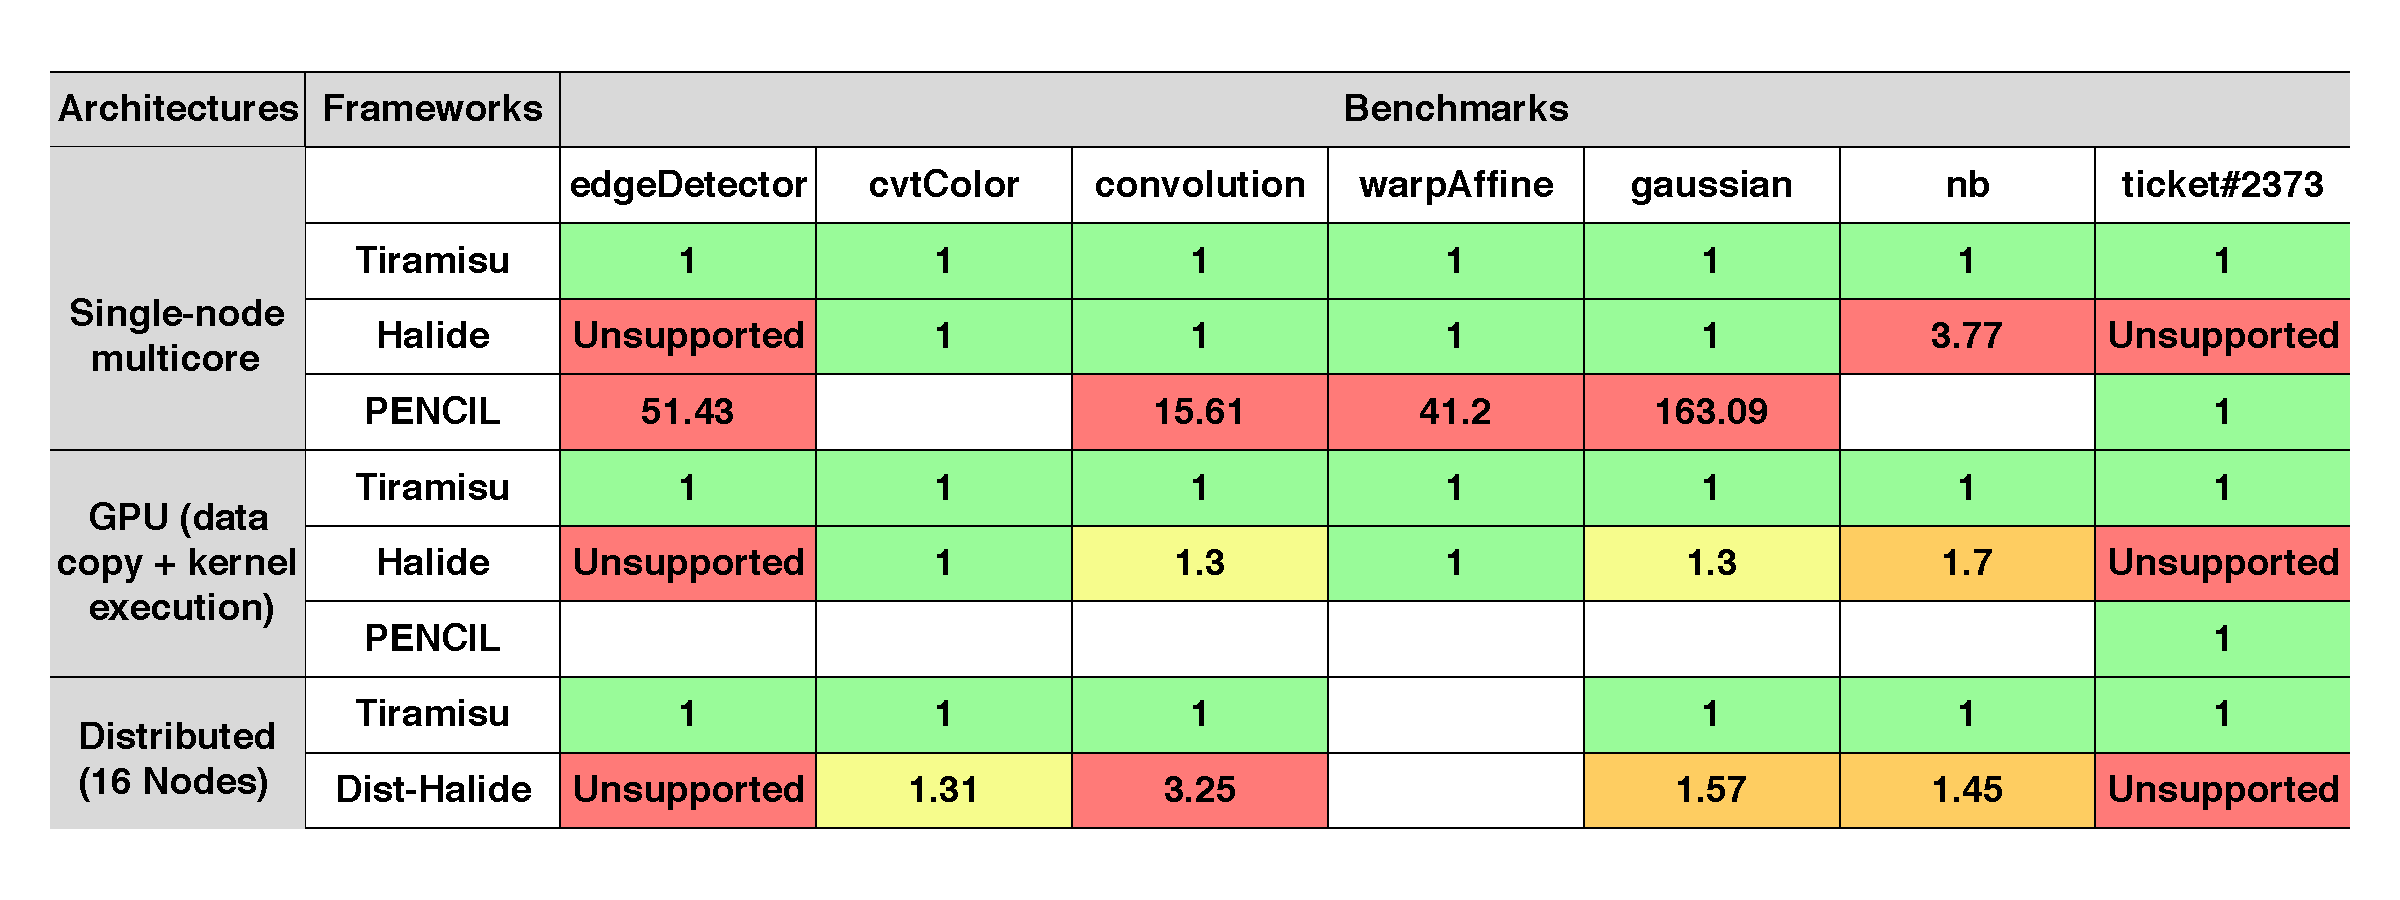
\includegraphics[width=1.05\columnwidth,trim=50 10 10 10]{./figures/tiramisu_heatmap.pdf}
\vspace{-0.5cm}
\caption{A heatmap comparing the normalized execution times of code generated by \framework{} with other frameworks (lower is better).  Comparison is performed on three architectures: single-node multicore, GPU, distributed (16 nodes).}
\label{fig:speedup}

\end{figure}

Figure~\ref{fig:speedup} compares the normalized execution time of code generated by \framework{} to other state-of-the-art frameworks on three architectures: single-node multicore, GPU and distributed (16 nodes).  For the single-node multicore and GPU we compare \framework{} to Halide, an industrial framework that uses a scheduling language, and to PENCIL, a fully automatic polyhedral compiler.  For the distributed architecture, we compare only to distributed Halide~\cite{denniston2016distributed} since PENCIL does not generate distributed code and the only other polyhedral compiler that generates distributed code (pluto-mpi) does not support non-affine code (4/7 of our benchmarks have non affine code).

\paragraph{Single-node multicore}
In four of the benchmarks, the performance of the code generated by \framework{} matches the performance of Halide.  We use the same schedule for both implementations; these schedules were hand-written by Halide experts.  The results for \texttt{edgeDetector}, \texttt{convolution}, \texttt{warpAffine} and \texttt{gaussian} which have non-affine array accesses and conditionals show that \framework{} handles such pattern efficiently.

Two of the other benchmarks, \texttt{edgeDetector} and \texttt{ticket \#2373}, cannot be implemented in Halide.  The following code snippet shows \texttt{edgeDetector}.
%is an example of a recurrent filter extracted from~\cite{recfilter}, a compiler designed to support recurrent filters.

\vspace{-0.15cm}
\begin{lstlisting}[language=C,escapechar=@,numbers=none]
/* Ring Blur Filter */
R(i,j) = (Img(i-1,j-1) + Img(i-1,j) + Img(i-1,j+1)+
          Img(i,j-1)   +              Img(i,j+1)  +
          Img(i+1,j-1) + Img(i+1,j) + Img(i+1,j+1))/8;
/* Roberts Edge Detection Filter */
Img(i,j) = abs(R(i,j)-R(i+1,j-1)) + abs(R(i+1,j)-R(i,j-1));
\end{lstlisting}
\vspace{-0.15cm}

\texttt{edgeDetector} cannot be implemented in Halide because it creates a cyclic dependence graph with a cycle length $\geq 1$.
Halide can only express programs with an acyclic dependence graph, with some exceptions;  this restriction is imposed by the Halide language and compiler to avoid the need to prove the legality of some optimizations (since proving the legality of certain optimizations is difficult in the Halide interval-based representation).
%in an interval-based representation in the case of a cyclic dependence graph.
\framework{} does not have this restriction since it checks transformation legality using dependence analysis~\cite{feautrier_dataflow_1991}.
%An other example of an a filter that exhibit this pattern include the PatchMatch algorithm~\cite{Barnes:2009:PRC:1531326.1531330}.
%By relying on dependence analysis to check the correctness of optimizations, \framework{} enables Halide to
%and on checking the legality of transformations using the polyhedral model~\cite{konrad_elimination_2011} to decide whether a transformation can be performed.

In \texttt{ticket \#2373}, which exhibits a triangular iteration domain,  Halide's bounds inference over-approximates the computed bounds which leads the generated code to fail in execution.  This over-approximation in Halide is due to the use of intervals to represent iteration domains, which prevents Halide from performing precise bounds inference for non-rectangular iteration spaces.  \framework{} can handle this case naturally since it relies on the polyhedral model where sets can include any affine constraint  in addition to loop bounds.  These examples show that the model exposed by \framework{} naturally supports more complicated code patterns than an advanced, mature DSL compiler.

For \texttt{nb}, the code generated from \framework{} achieves $3.77\times$ speedup over the Halide-generated code. This is primarily due to loop fusion.  In this code, \framework{} enhances data locality by fusing loops into one loop;  this is not possible in Halide, which cannot fuse loops if they update the same buffer.  Halide makes this conservative assumption because otherwise it cannot prove the fusion is correct. This is not the case for \framework{} which uses dependence analysis to prove correctness.

In comparison with PENCIL, the main difference is that both \framework{} and Halide apply vectorization and unrolling on the innermost loops while PENCIL does not.  Most of the benchmarks have many statements within the innermost loop, therefore vetorizing the innermost loop transforms all of those statements to their vector equivalent while unrolling increases register reuse and instruction level parallelism.

\paragraph{GPU}
For the GPU backend, the reported times are the total execution times (data copy and kernel execution).
Code generated by \framework{} for \texttt{convolution} and \texttt{gaussian} is faster than that of Halide because code generated by \framework{} uses constant memory to store the weights array, while the current version of Halide does not use constant memory for its PTX backend.  The only different between the schedule of \framework{} and Halide in these benchmarks is the use of \texttt{tag\_gpu\_constant()} in \framework{}.  Data copy times, for all the filters,  are the same for \framework{} and Halide.

In comparison with PENCIL ...

\begin{figure}[t]
\centering
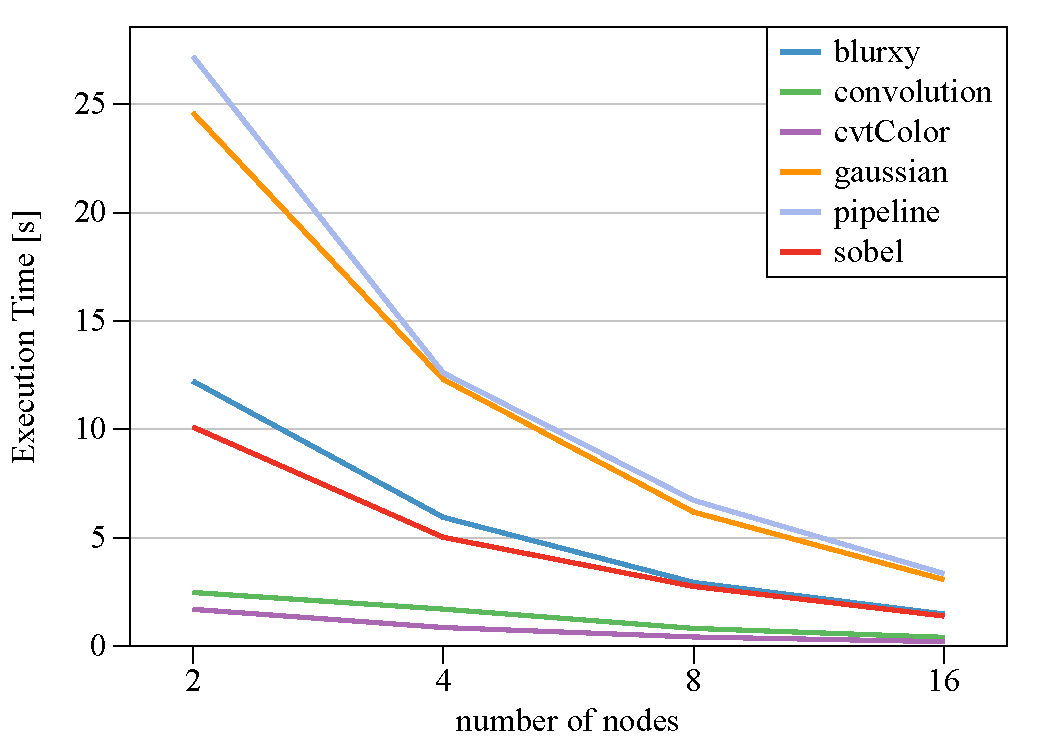
\includegraphics[width=0.6\columnwidth, trim=0 30 0 60]{./figures/tiramisudist}
\caption{Execution time of distributed \framework{} for 2, 4, 8, and 16 nodes}
\label{fig:distCPU_tiramisu_scaling_exec}
%\vspace{-0.5cm}
\end{figure}

\paragraph{Distributed}
We assume the data are already distributed across the nodes by rows. Of these benchmarks, \texttt{nb}, \texttt{cvtColor} and \texttt{ticket \#2373} do not require any communication; the other four require communication due to overlapping boundary regions in the distributed data.

Figure \ref{fig:speedup} compares the execution time of distributed \framework{} and distributed Halide. \framework{} is faster than distributed Halide in each case. For the kernels involving communication, code generated by distributed Halide has two problems compared to \framework{}:  distributed Halide overestimates the amount of data it needs to send, and unnecessarily packs together contiguous data into a separate buffer before sending.  %jHalide distributed always packs the data that need to be sent into a buffer then sends the data (this strategy is useful for the general case but is not needed in this case).

The only difference between the \framework{} and distributed Halide code for these benchmarks is the use of the \texttt{send} and \texttt{receive} scheduling commands in \framework{}.  These commands allow the user to specify exactly the amount of data to send and also allow the compiler to avoid unnecessary packing.
%In addition to this, in \framework{}, the user specifies exactly which data should be transferred between nodes so there is no additional run-time overhead.  For the kernels not requiring communication, Halide still has to fully check that the data to send is an empty set (the interval model used in Halide does not allow compile-time emptiness check).

Figure \ref{fig:distCPU_tiramisu_scaling_exec} shows the execution time of the kernels with distributed \framework{} when running on 2, 4, 8, and 16 nodes.  This graph shows that distributed code generated from \framework{} scales well as the number of nodes increases (strong scaling).

\vspace{-0.25cm}
\subsection{Evaluation Summary}

Overall, the experiments demonstrate the use of \framework as an optimization framework for implementing a set of image processing kernels and stencils, for multiple backends.  We show that \framework{} is expressive: it enables implementng new optimizations and algorithms not supported by Halide.  The experiments also show that \framework{} is suitable for targeting multiple hardware architectures, including multicore CPUs, GPUs and distributed systems. Thanks to its flexible scheduling commands, it generates highly optimized code for a variety of of architectures and algorithms.
